\section{Auswertung}
\label{sec:Auswertung}
\subsection{Schwellenstrom}
Wie in Kapittel \ref{sec:Lasergranulation} beschrieben,
wird der Schwellenstrom mithilfe der Lasergranulation bestimmt.
\begin{figure}[h]
    \centering
    \begin{minipage}[t]{0.45\textwidth}
        \centering
        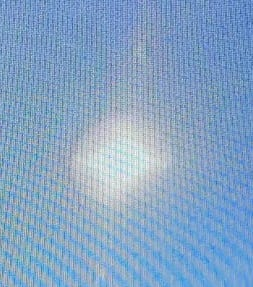
\includegraphics[width=1\linewidth]{abb/LED.jpeg}
    \end{minipage}
    \begin{minipage}[t]{0.45\textwidth}
        \centering
        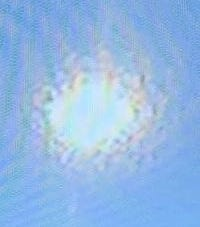
\includegraphics[width=1\linewidth]{abb/Lasergranulation.jpeg}
    \end{minipage}
    \caption{Übergang von LED zu Laser Licht}
    \label{fig:Strom}
\end{figure}
Der Übergang tritt bei einem Schwellenstrom von $34.5$mA ein und ist in Abbildung \ref{fig:Strom} dargestellt.

\subsection{Rubidiumfluoreszenz und das Transmissionsspektrum}
Die beim einstellen des Aufbaus erforderliche Rubidiumfluoreszenz ist in Abbildung \ref{fig:Fluoresenz} dargestellt.
\begin{figure}[h]
    \centering
    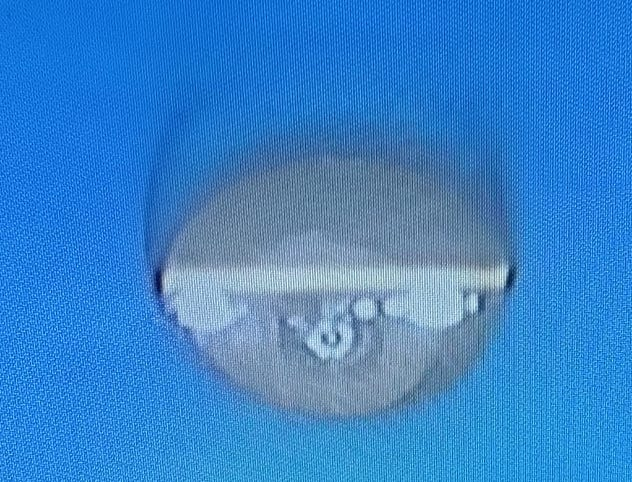
\includegraphics[width=0.4\textwidth]{abb/Fluresenz.jpeg}
    \caption{Rubidiumflureszenz}
    \label{fig:Fluoresenz}
\end{figure}
Nach dem eliminieren der Auftretenden Mode Hops ergibt sich der in  Abbildung \ref{fig:graph} dargestellte Graph.
Es sind deutlich die vier zu erwartenden Peaks zu erkennen.
Von Links nach rechts die Übergänge 87a,85a,85b,87b.
\begin{figure}[h]
    \centering
    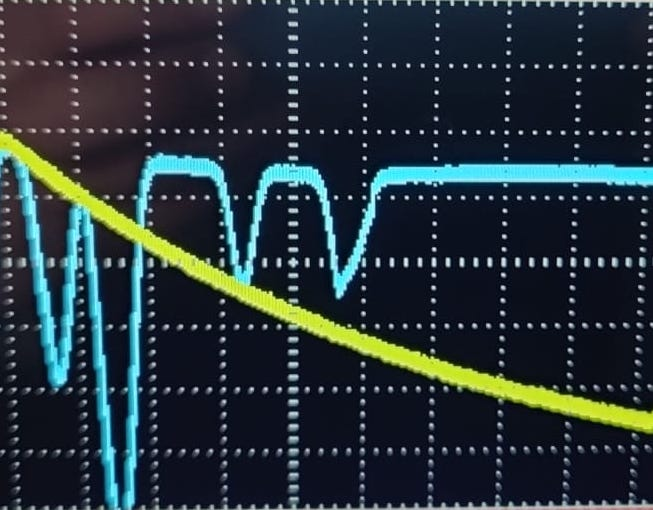
\includegraphics[width=0.6\textwidth]{abb/Graph.jpeg}
    \caption{Transmissionsspektrum von Rubidium}
    \label{fig:graph}
\end{figure}